\section{Paper 10}
\subsection{\emph{"Convolutional Neural Networks for Risso’s Dolphins Identification"}}

\begin{frame}{INTRODUCTION}
    Photo identification is a technique that can be used on marine species in 
    order to safeguard the environment and the various existing species. The 
    marine species on which this study is based are cetaceans, in particular the 
    Risso's dolphin species Grampus Griseus (Fig. \ref{fig:Risso}). In order to 
    recognize a dolphin, the scars present on their body and on the dorsal fin are 
    used, representing the "fingerprints" useful for identifying them. To 
    achieve this, a new network model called NNPool is introduced.
    \begin{figure}[h!]
        \centering
        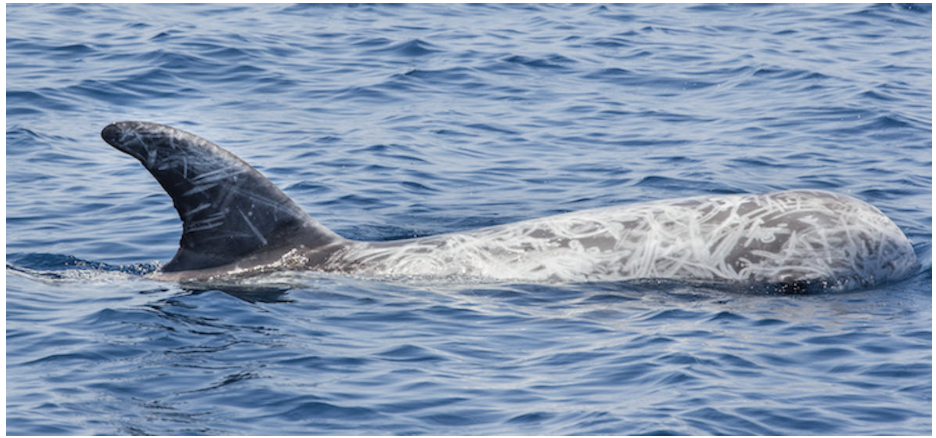
\includegraphics[width = 0.5\linewidth]{images/paper10/Risso.png}
        \centering
        \caption{Risso’s dolphins Grampus Griseus}
        \label{fig:Risso}
    \end{figure}
\end{frame}

\begin{frame}{MATERIAL AND METHODS}
    The following work comes from the evolution of two other previously 
    created methods that use two different classification algorithms: 
    \emph{RUSBoost} \footfullcite{0907875812} and \emph{RUSPool}\footfullcite[]{0907875814}. Each model, including the one proposed, is 
    trained on a specific dataset, each of which represents the update of the 
    other. The datasets are as follows:
    \begin{enumerate}
        \item $D_R$: consisting of 433 images, used for training RUSBoost method;
        \item $D_V$: consisting of 300 images, used for training RUSPool method;
        \item $D_{NN}$: consisting of 582 images, used for training NNPool method;
    \end{enumerate}
    Each dataset contains more than one image belonging to the single 
    dolphin. Each of them is divided into training sets and test sets of 
    labeled images.
\end{frame}

\begin{frame}{MATERIAL AND METHODS - RUSBoost}
    \begin{minipage}{\linewidth}
        \centering
        \begin{minipage}{0.47\linewidth}
            RUSBoost consists of two other types of algorithms: Random Under-Sampling 
            (RUS) and Adaboost. RUSBoost training takes place by carrying out 
            cross-validation, one against all, on each of the 23 dolphins taken into consideration.
            \begin{enumerate}
                \item \emph{Pre-processing}: creation of the black and white image containing the 
                extracted fin.
                \item \emph{Features Extraction}: build the 3-dimensional super-SIFT descriptor. 
                \item \emph{Classification}: application of the RUSBoost algorithm.
            \end{enumerate}  
        \end{minipage}
        \hspace{0.05\linewidth}
        \begin{minipage}{0.45\linewidth}
            \begin{figure}[h!]
                \centering
                \includegraphics[width =\linewidth]{images/paper10/RUSBoost model.png}
                \centering
            \end{figure}
        \end{minipage}
    \end{minipage}
\end{frame}

\begin{frame}{MATERIAL AND METHODS - RUSPool}
    The RUSPool algorithm aims to identify known dolphins among all and unknown 
    ones. This task is done by using the previous 23 already trained 
    RUSBoosts classifiers. Therefore, each image given as input to RUSPool 
    will have n super-SIFT descriptors associated with it and this new sample is 
    supplied as input to the RUSBoosts classifiers. The result returned by each 
    classifier will represent the prediction that a dolphin has been recognized or 
    not.In the output vector $R$, if there is an $r_i$ greater than a certain threshold, then the dolphin will be classified as known.
    \begin{minipage}{\linewidth}
        \centering
        \begin{minipage}{0.47\linewidth}
            \begin{figure}[h!]
                \centering
                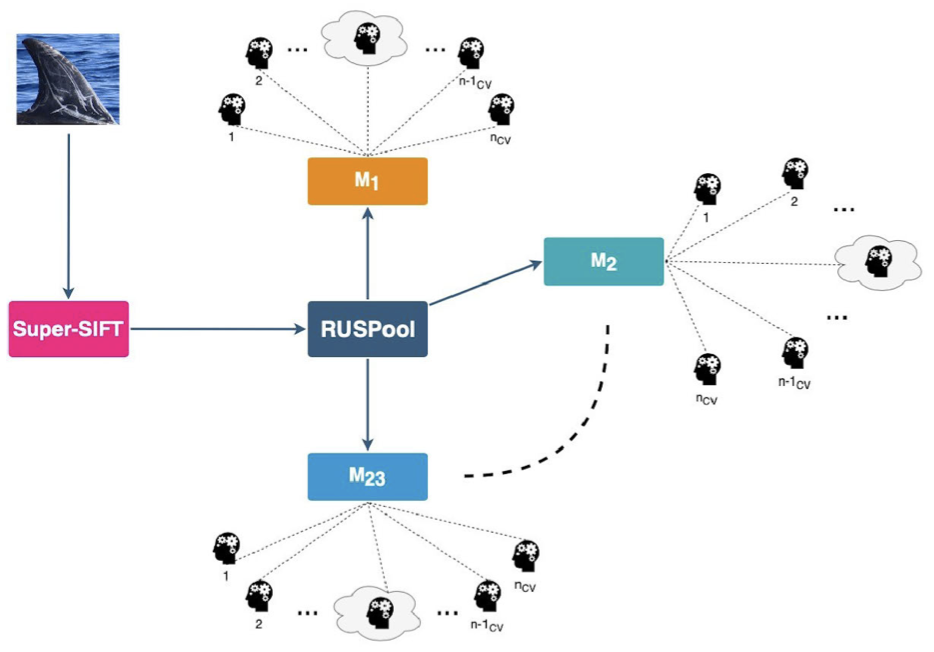
\includegraphics[width =\linewidth]{images/paper10/RUSPool Architecture.png}
                \centering
            \end{figure}
        \end{minipage}
        \hspace{0.05\linewidth}
        \begin{minipage}{0.45\linewidth}
            \begin{figure}[h!]
                \centering
                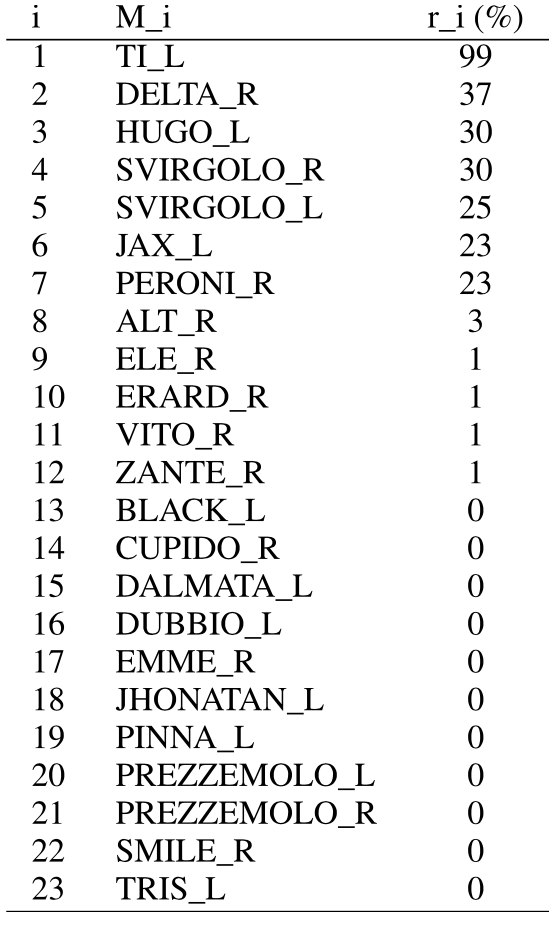
\includegraphics[width = 0.5\linewidth]{images/paper10/ri.png}
                \centering
            \end{figure}
        \end{minipage}
    \end{minipage}
    
\end{frame}

\begin{frame}{MATERIAL AND METHODS - NNPool}
    The proposed network architecture consists of 28 CNN networks, each of which is trained in recognizing a specific dolphin. If there is a single probability $p_i\in P > 51\%$ in the output vector $P$, then this input dolphin will be classified as known. Each song on the CNN network has the following architecture:
    \begin{minipage}{\linewidth}
        \centering
        \begin{minipage}{0.47\linewidth}
            \begin{figure}[h!]
                \centering
                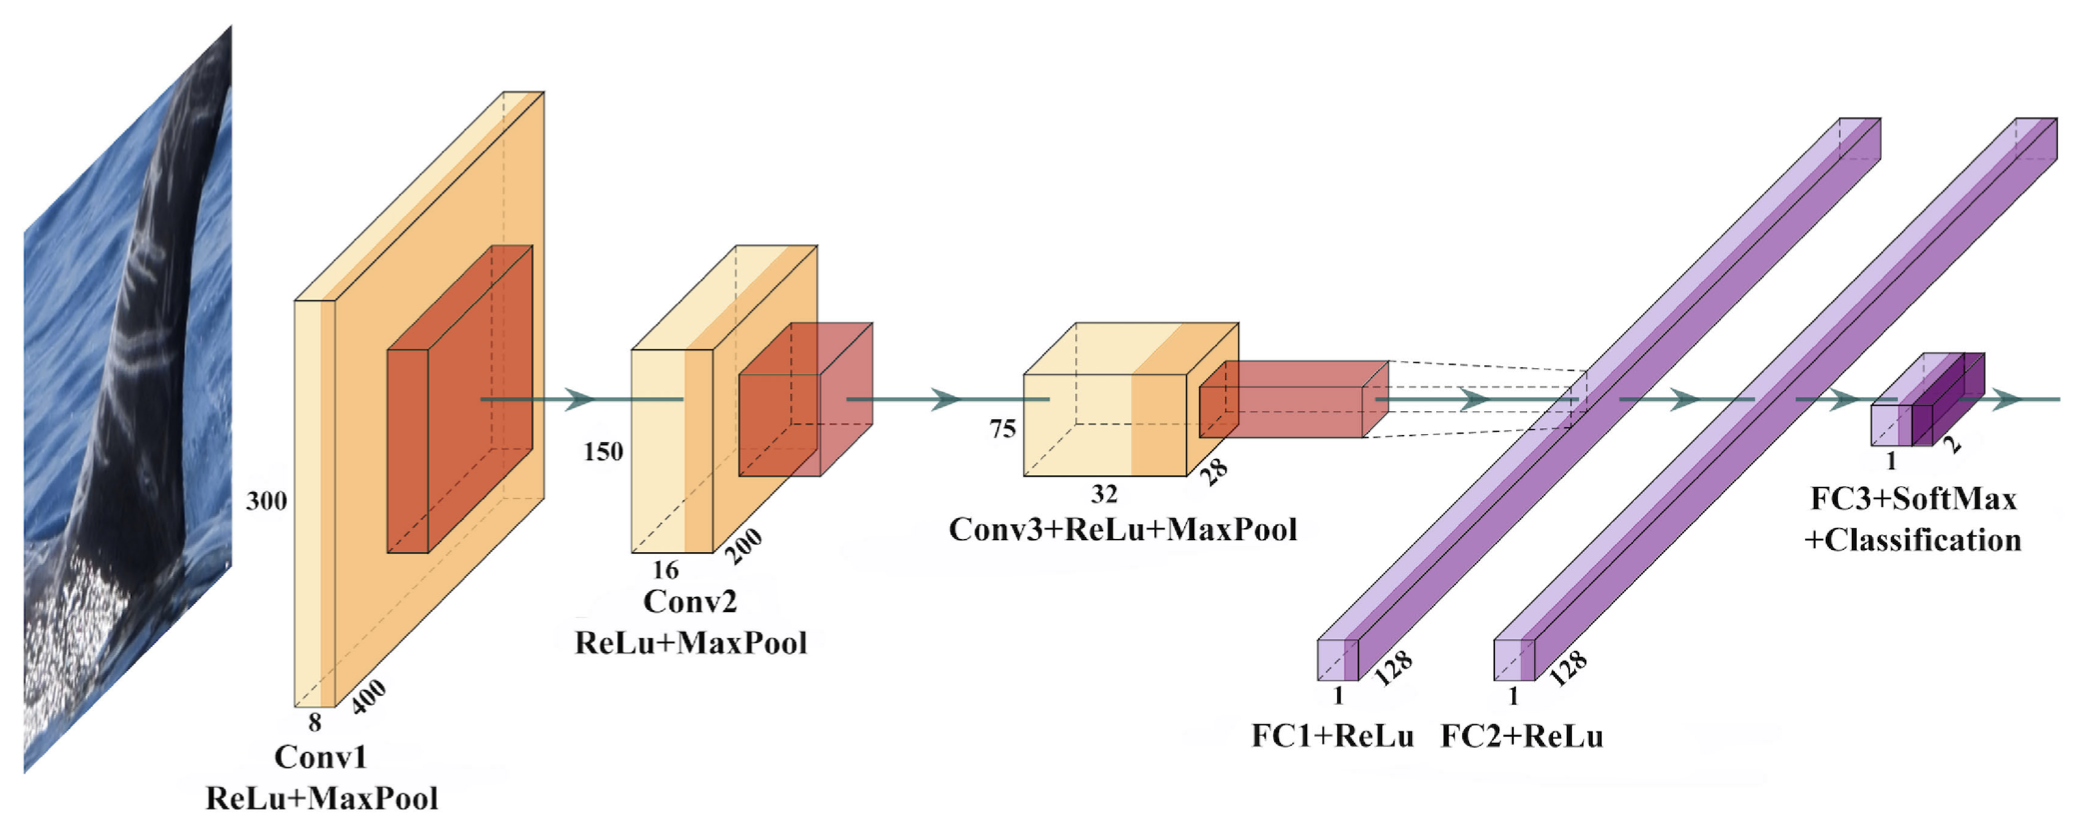
\includegraphics[width = \linewidth]{images/paper10/NNPool Architecture.png}
                \centering
                \caption{CNN Architecture build for each dolphin.}
                \label{fig:CNNDol}
            \end{figure} 
        \end{minipage}
        \hspace{0.05\linewidth}
        \begin{minipage}{0.45\linewidth}
            \begin{figure}[h!]
                \centering
                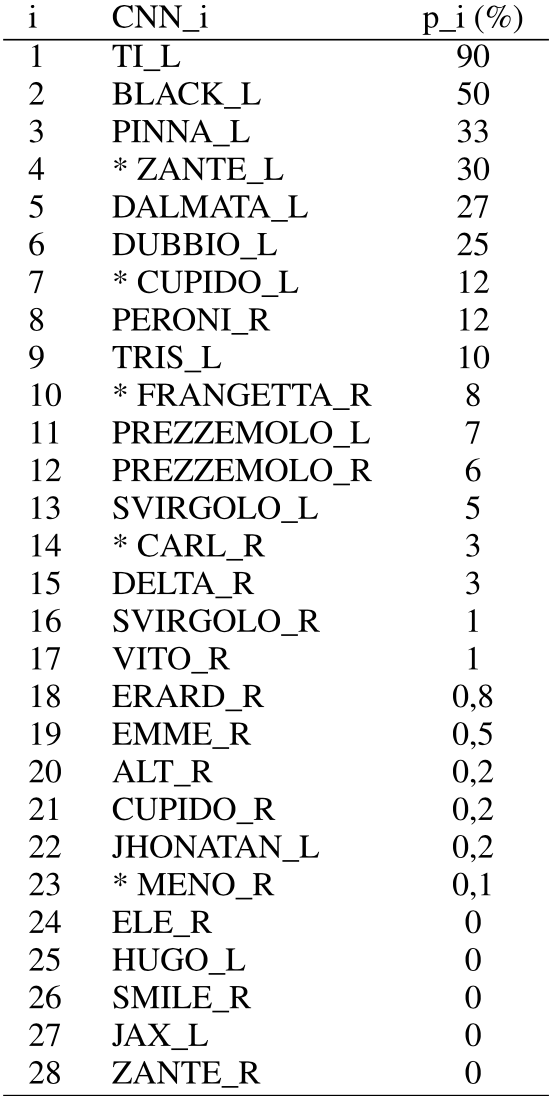
\includegraphics[width = 0.5\linewidth]{images/paper10/NNPool output.png}
                \centering
            \end{figure}
        \end{minipage}
    \end{minipage}    
\end{frame}

\begin{frame}{EXPERIMENTS AND RESULTS - Metrics}
    The metrics used to evaluate the performance of the proposed model are as follows:
    \begin{enumerate}
        \item \emph{Accuracy}: percentage of correct predictions.
        \item \emph{Sensitivity}: percentage of positive labels considered as positive.
        \item \emph{Specificity}: percentage of negative labels considered as negative.
        \item \emph{PIQE}: determines the type of quality (Excellent, Good, Fair, Poor, Bad) (Low score is better).
    \end{enumerate}
    Images labeled as negative will correspond to unknown classes.
\end{frame}

\begin{frame}{EXPERIMENTS AND RESULTS - RUSPool Vs. NNPool}
    \begin{minipage}{\linewidth}
        \centering
        \begin{minipage}{0.45\linewidth}
            \begin{figure}[h!]
                \centering
                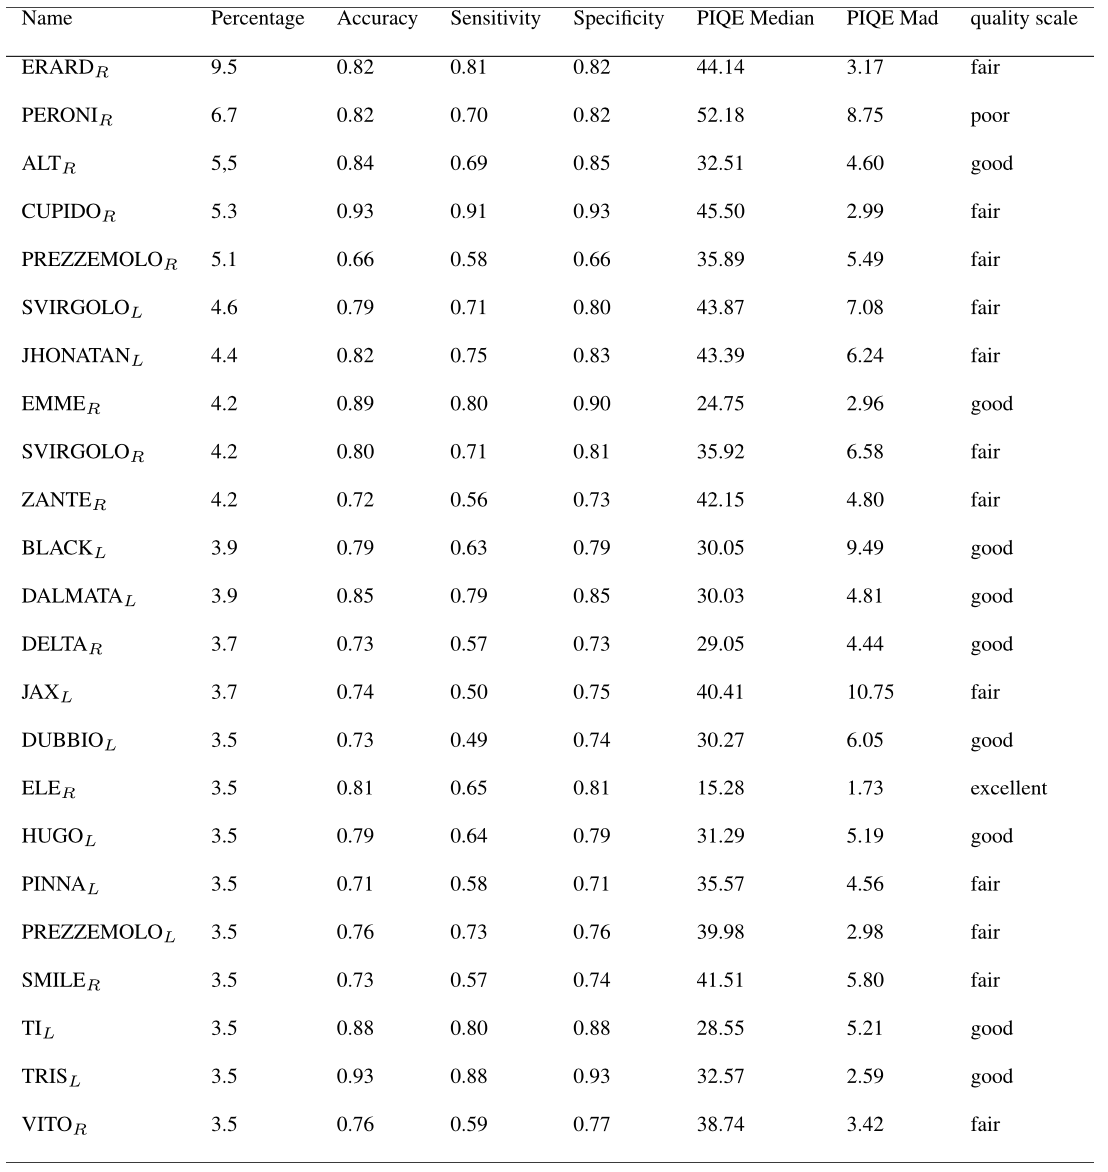
\includegraphics[width = \linewidth]{images/paper10/RUSBoost performance.png}
                \centering
                \caption{Performances of every RUSBoost classifiers in RUSPool method.}
                \label{fig: RUSBoostPerf}
            \end{figure}
        \end{minipage}
        \hspace{0.05\linewidth}
        \begin{minipage}{0.45\linewidth}
            \begin{figure}[h!]
                \centering
                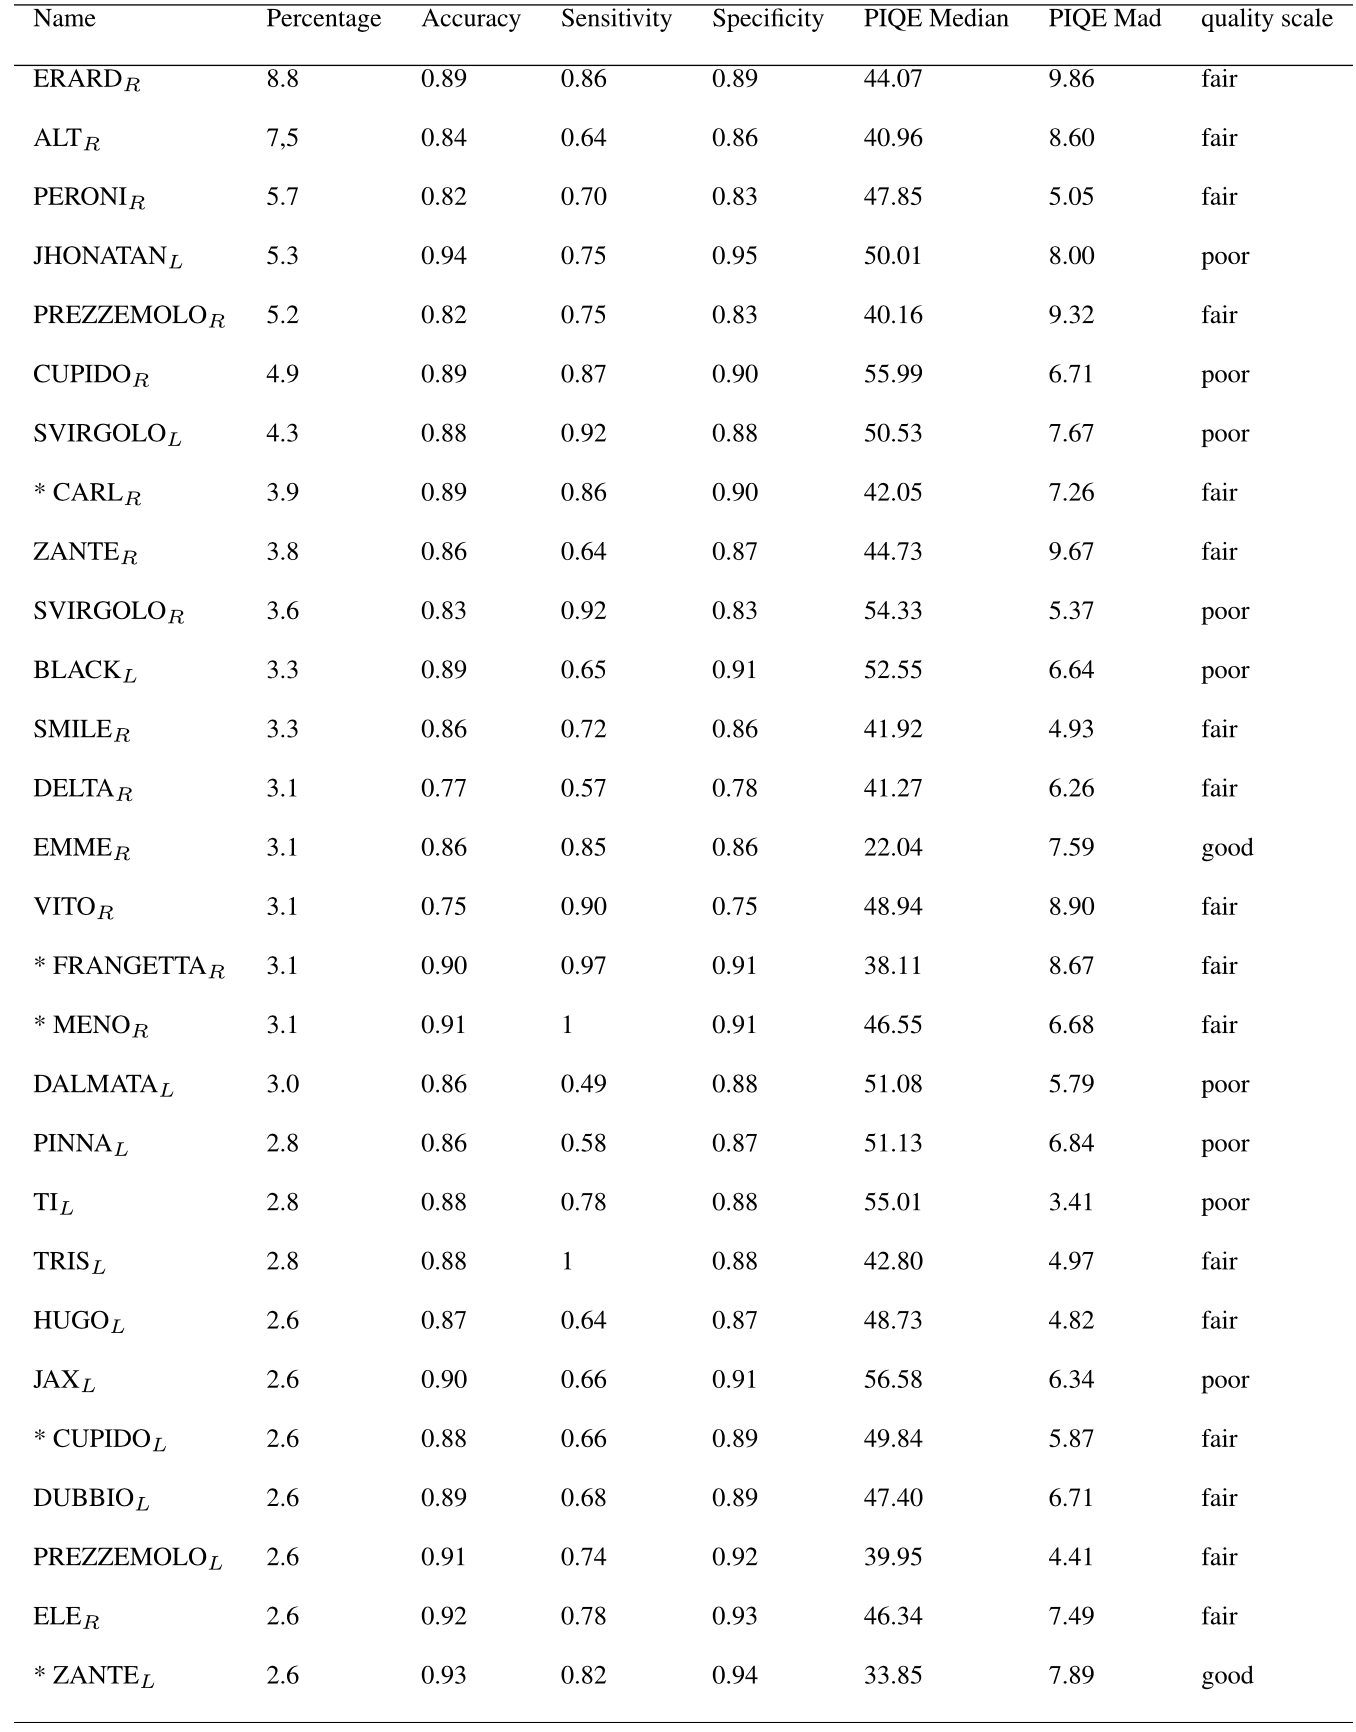
\includegraphics[width =\linewidth]{images/paper10/NNPool performance.png}
                \centering
                \caption{Performances of every CNN network in NNPool method.}
                \label{fig: CNNNNPool perfromance}
            \end{figure}
        \end{minipage}
    \end{minipage}   
\end{frame}

\begin{frame}{CONCLUSION}
    In conclusion, it can be said that, among all the methods compared, the 
    proposed CNN network has better performances and more advantages. 
    One of the first is the non-interaction of the user, while following there is 
    the factor of the training and classification speed. Even having better 
    performance than RUSPool (Tab. \ref{RUSPoolPerf}), NNPool's CNNs networks have the 
    problem of the number of images and their quality, in fact by providing a 
    low number of images, all with low quality, the proposed algorithm will 
    tend to have low performance in terms classification of dolphins. The 
    strong point of the CNN network is that it achieves good performance 
    both in case there are many low quality images and in case there are few 
    high quality images.
    \begin{table}[htbp]
        \centering
        \begin{adjustbox}{width=0.6\textwidth}
        \begin{tabular}{|cccc|}
            \hline
            & Accuracy & Sensitivity & Specificity\\
            \hline
            RUSPool & 0.78 & 0.58 & 0.81\\
            NNPool & 0.87 & 0.70 & 0.90\\
            \hline
        \end{tabular}
        \end{adjustbox}
        \caption{RUSPool and NNPool performance.}
        \label{RUSPoolPerf}
    \end{table}
\end{frame}